\chapter{ALTERNATE CONTROL SAMPLE FOR QCD BACKGROUND ESTIMATION}
\label{app:ee}
In the analysis performed using the 2015 CMS data set~\cite{CMS:2015_anal}, 
a sample of $Z\rightarrow ee$ events (referred to as the $ee$ sample) was used as the 
primary QCD background estimate, and the $ff$ control 
sample was used to set a systematic uncertainty on the background.
The idea was that the $ee$ and $ff$ control samples represent
100$\%$ and 0$\%$ photon purity, respectively. By using both, we could
derive a bound on any possible sensitivity of the \ETmiss spectrum
to the object purity. 

\section{Problems with using $ee$}
\label{sec:eeProblems}
There are several reasons we decided not to use the $ee$ control sample
 in the 2016 analysis. One reason was uncertainty on 
 the efficiency of the control 
 trigger. As mentioned in Chapter~\ref{chap:Trigger},
the primary analysis trigger 
cannot be used due to the $m_{\gamma\gamma}~<~90~GeV$
invariant mass requirement. Instead, the $ee$ sample uses the control trigger 
listed in Table~\ref{tab:triggers}. As shown in~\ref{sec:eeEff}, the
control trigger is only 79.8\% efficient because it 
requires both electromagnetic objects to be matched to a 
pixel seed. There is a relatively 
large uncertainty on this efficiency because of its
slow turn-on. Our offline photon \pT threshold of 40 GeV is 
barely in the plateau, and the trigger continues to get more efficient 
as \pT increases. 

Another reason why we prefer $ff$ over $ee$ is that the kinematics
of $ff$ are more similar to the kinematics of our SUSY signal events.
In $ee$ events, the the two electromagnetic objects are obviously correlated, 
since they come from the decay of the $Z$ boson. In the $ff$ and SUSY diphoton
events, on the other hand, the photons and fakes are uncorrelated. The result
is that the $ee$ and $\gamma\gamma$ \ETmiss distributions start to diverge
once the statistical uncertainties do down. 

The most significant reason for not using $ee$, was actually 
not the trigger or kinematics, but large contributions from processes with real \ETmiss 
 such as $t\bar{t}$ and $ZZ\rightarrow ee\nu\nu$. 
The idea of the QCD background estimation method is that we 
select control samples that do not have inherent \ETmiss. 
For the case of $ee$, however,
there are processes with inherent \ETmiss that contaminate
the sample. 
In \ttbar events where both tops decay leptonically,
there can be final states with two electrons and
multiple neutrinos. Similarly, $ZZ \rightarrow ee\nu\nu$
events will fall into our $ee$ category.
These contributions are modeled with MC and subtracted 
from the $ee$ distribution in data. 
The MC samples used are listed in
Table~\ref{tab:eeDatasets}.

\begin{table}[ht]
  \caption{BACKGROUND MC SAMPLES FOR EE SAMPLE}
  \centering
  \begin{tabular}{|>{\centering\arraybackslash}m{0.9\linewidth}|}
    \hline
    \hline
    /TT$\_$TuneCUETP8M2T4$\_$13TeV-powheg-pythia8/
    RunIISummer16MiniAODv2-PUMoriond17$\_$ 
    80X$\_$mcRun2$\_$asymptotic$\_$2016$\_$TrancheIV$\_$v6-v1/MINIAODSIM\\
    \hline
    /ZZTo2L2Nu$\_$13TeV$\_$powheg$\_$pythia8/
    RunIISummer16MiniAODv2-PUMoriond17$\_$ 
    80X$\_$mcRun2$\_$asymptotic$\_$2016$\_$TrancheIV$\_$v6-v1/MINIAODSIM\\
    \hline
    \hline
    \end{tabular}
    \label{tab:eeDatasets}
     \justify{MC samples used to remove contributions
     to the $ee$
    control sample
    from processes with real \ETmiss.}
\end{table}

Table~\ref{tab:subtract} shows the percent contribution
from these processes in the signal region. In some bins, 
95\% of the observed $ee$ events can be attributed to 
these real-\ETmiss processes.
As you can see in Figure~\ref{fig:eeWeighted},
very few $ee$ events remain in the tail after 
performing this subtraction.


\begin{table}[ht]
     \caption{Contribution to the $ee$ sample from processes with real \ETmiss}
     \centering % used for centering table                                                                                                                    
     \begin{tabular}{| c | c | c |} % centered columns (4 columns)                                                                                            
    \hline
     \ETmiss bin (GeV) & \ttbar Contribution & ZZ Contribution\\ [0.5ex]
     \hline
     $100-115$ & 58.8\% & 3.9\% \\
     $115-130$ & 87.4\% & 6.6\% \\
     $130-150$ & 87.3\% & 8.1\% \\
     $150-185$ & 86.7\% & 10.4\% \\
     $185-250$ & 64.2\% & 15.2\% \\
     $~>~250$  & 45.8\% & 22.6\% \\
     \hline
     \end{tabular}
     \label{tab:subtract}
\end{table}

%\subsection{Systematic uncertainties on \ttbar subtraction}
%\label{sec:ttbarUncert}

For the subtraction of $ZZ \rightarrow ee\nu\nu$ events, 
we consider uncertainties from
MC statistics and jet energy scale corrections.
Both uncertainties are less than a 2\% effect
on the final $ee$ estimate in the signal region.

The systematic uncertainties associated with 
the subtraction of the \ttbar contribution to the $ee$ control
sample are much more significant. 
Because we are subtracting a large majority of the
original $ee$ events at high \ETmiss, the relative
uncertainties on the expected number of \ttbar events get inflated.
In the signal region, the limited MC \ttbar statistics
leads to an uncertainty of up to 140\%. Uncertainties
from the parton distribution function and overall
scale of the cross section lead to uncertainties
on the final $ee$ estimate up to 94\%.
Jet energy scale corrections
of the \ttbar sample lead to uncertainties up to
97\%, and the effect of reweighting by the
top \pt to correct for differences between
MC and data is up to 70\%.

The large corrections and associated uncertainties
to make the $ee$ sample representative of the
events we were trying to model
was the primary reason why we ultimately
decided not to use the $ee$ control sample for the
QCD background estimate.

%%%%%%%%%%%%%%%%%%%%%%%%%%%%%%%%%%%%%%%
%%%%%%%%%%%%%%%%%%%%%%%%%%%%%%%%%%%%%%%

\section{Results using ee sample}
\label{sec:eeResults}
As was done for the $ff$ sample,
any difference in hadronic activity between the control and candidate
samples needs to be corrected.
This includes differences in hadronic
activity as modeled by the di-EM \pt variable, but also includes
differences in the jet multiplicity distributions.
For example, the energy resolution in an event where
there are three jets having a total \pt of $100$ GeV will be worse than that
of an event where there is only one jet with \pt of $100$ GeV.
Figure~\ref{fig:eediEMPTRatio} shows a
comparison of the $ee$ and $\gamma\gamma$ di-EM \pt distributions, and
the jet multiplicity distributions are shown in Figure~\ref{fig:JetDistribution1D}.
The jet multiplicity distributions for the candidate and $ff$ samples are
similar, but the candidate and $ee$ distributions are noticeably different.
%%
%%\begin{figure}[h]
%%\begin{center}
%%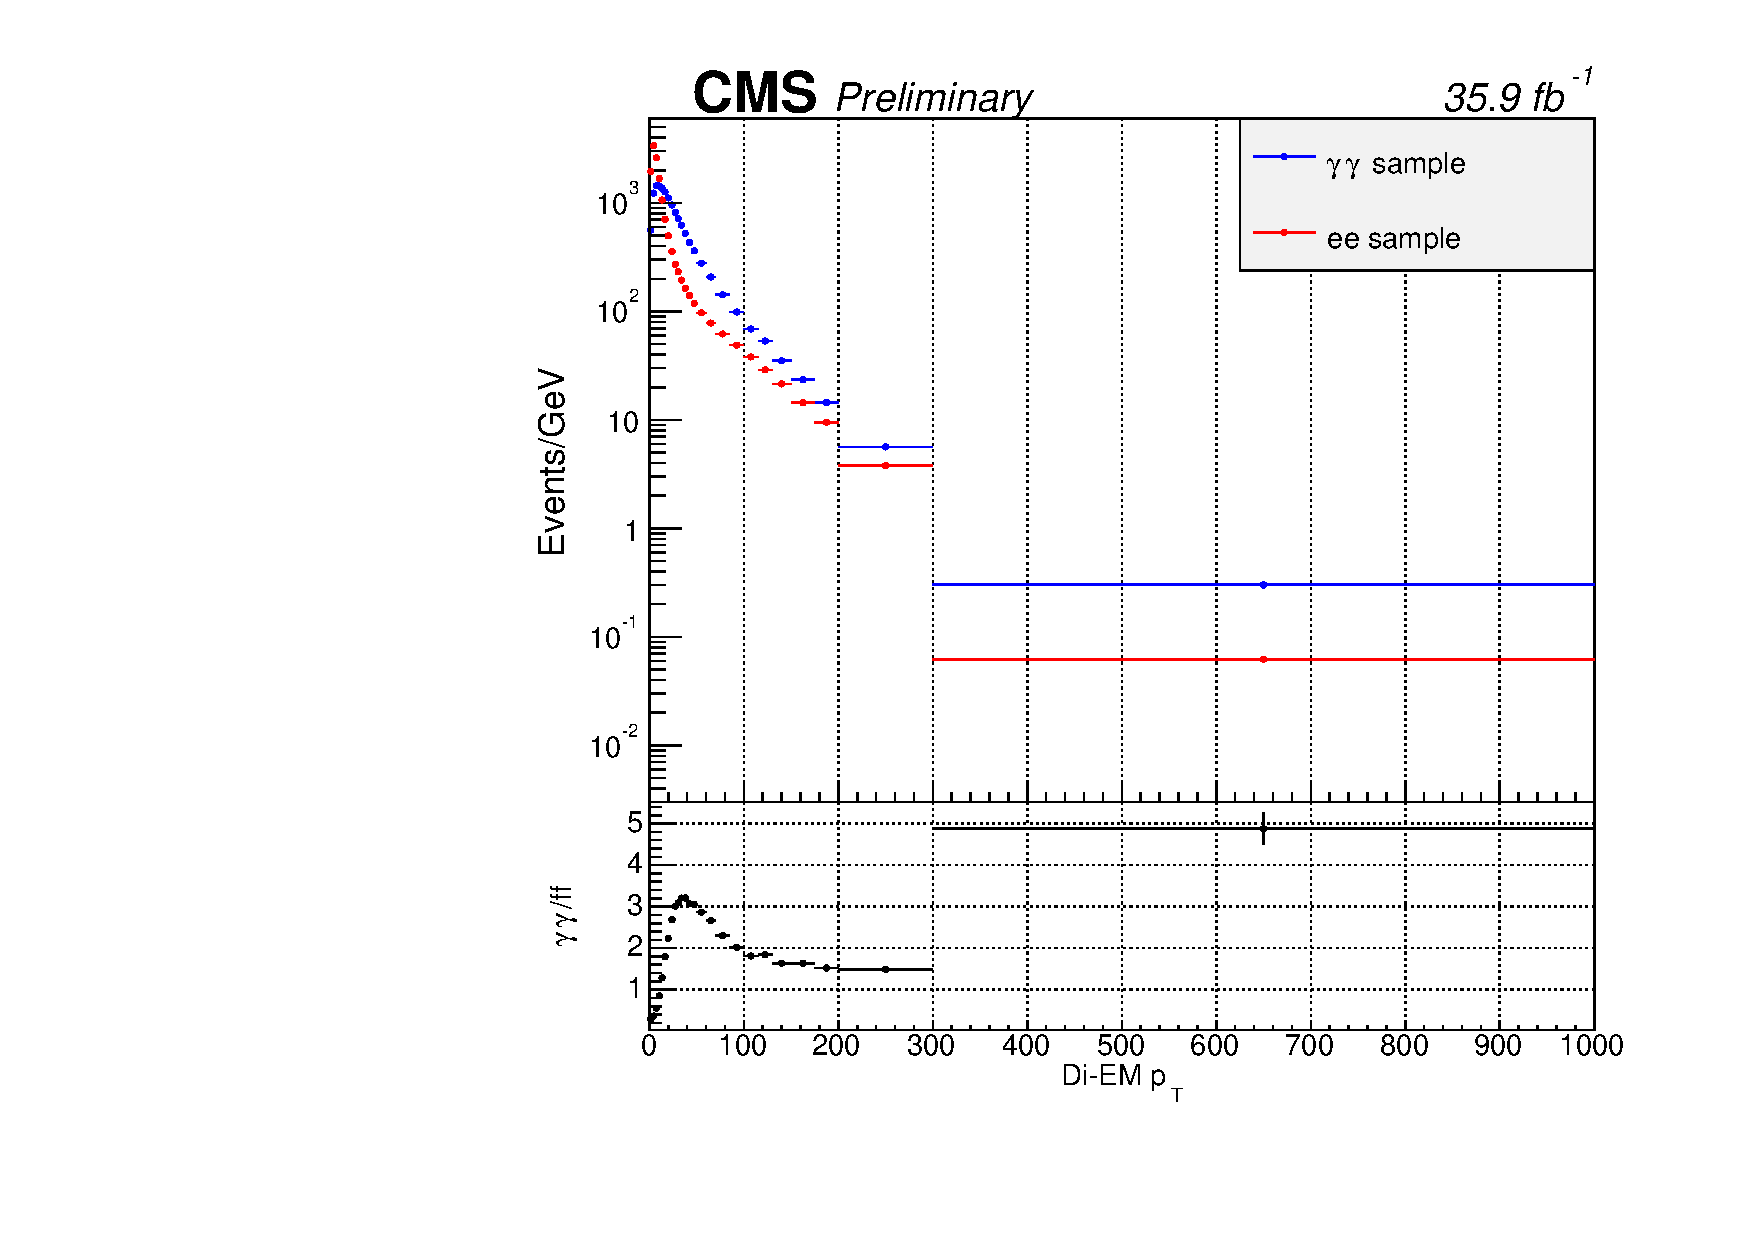
\includegraphics[width=4.0in]{figs/eeDiempt.pdf}
%%\end{center}
%%\caption{Comparison of di-EM \pt distributions of $\gamma\gamma$ and $ee$ samples.}
%%\label{fig:eediEMPTRatio}
%%\end{figure}
%%
%%
%%\begin{figure}
%%\begin{center}
%% \includegraphics[width=6.0in]{figs/JetMultiplicity.pdf}
%% \end{center}
%% \caption{Jet multiplicity distributions of the candidate, $ee$ and $ff$ samples.}
%% \label{fig:JetDistribution1D}
%%\end{figure}
%
%To account for any possible dependence between the di-EM \pt and the
%jet multiplicity, the $ee$ sample was reweighted by the ratio of
%$\gamma\gamma$ over $ee$ in bins of jet multiplicity versus
%di-EM \pt. The reweighting factors are shown in Figure \ref{fig:JetDistribution2D}.
%Figure~\ref{fig:eeReweighting} shows the effect of reweighting
%the $ee$ control sample by di-EM \pt only or by reweighting the
%$ee$ \ETmiss distribution by
%the jet multiplicity in bins of di-EM \pt.
%
%%\begin{figure}
%%\begin{center}
%% \includegraphics[width=6.0in]{figs/NJetVsDiempt.pdf}
%% \end{center}
%% \caption{$\gamma\gamma$ over $ee$ jet multiplicity distribution ratio in bins of di-EM \pt.}
%% \label{fig:JetDistribution2D}
%%\end{figure}
%%
%%\begin{figure}
%%\begin{center}
%% \includegraphics[width=6.0in]{figs/NJetMetCompare.pdf}
%% \end{center}
%% \caption{\ETmiss distributions for the $ee$ sample reweighted by di-EM \pt only (red) and the $ee$ sample reweighted by the 2D distribution of di-EM
%%\pt vs jet multiplicity (black). The ratio plot shows the ratio of red points to black points.}
%% \label{fig:eeReweighting}
%%\end{figure}
%
%A comparison of the unweighted \ETmiss distributions for the $ee$ and
%$ff$ control samples and the $\gamma\gamma$ candidate sample
%is shown in Figure \ref{fig:eeUnweighted}. The comparison after
%the reweighting procedure is shown in Figure~\ref{fig:eeWeighted}.
%
%%\begin{figure}[h]
%%\begin{center}
%%\includegraphics[width=6.0in]{figs/eeUnweightedMet.pdf}
%%\end{center}
%%\caption{Unweighted \ETmiss distributions of the $ee$ and $ff$ control samples and the $\gamma\gamma$ candidate sample.
%%The $ee$ and $ff$ distributions have been normalized to the \ETmiss$<50$ GeV region of the candidate sample.}
%%\label{fig:eeUnweighted}
%%\end{figure}
%%
%%\begin{figure}[h]
%%\begin{center}
%%\includegraphics[width=6.0in]{figs/eeReweightedMet.pdf}
%%\end{center}
%%\caption{\ETmiss distributions of the candidate sample, the reweighted $ee$ sample and the reweighted $ff$ sample.
%%The $ee$ and $ff$ distributions have been normalized to the \ETmiss$<50$ GeV region of the candidate sample.}
%%\label{fig:eeWeighted}
%%\end{figure}
%
